\section{Optimizer Parameters}

\subsection{Stripe Granularity}
The number of stripes is a parameter in the optimizer that determines the unit of data size that the optimizer determines routes. Choosing too small a number of stripes (e.g., 1-4) can result in solution infeasibility, since an individual stripe may be too large to fit along any given link under a replication time constraint.
% \ion{Why is that? In fact capacity and stripe size are not even comparable, one is measured in Gbps, and the other one in GB!} 
We show the tradeoff in \ref{fig:stripe-quality} between solution quality (dollar cost) and the number of stripes set of solving a 3-destination topology. Adding more stripes can increase the solver runtime unnecessarily. We use $8-16$ stripes for experiments. 

\begin{figure}[ht]
    \centering
    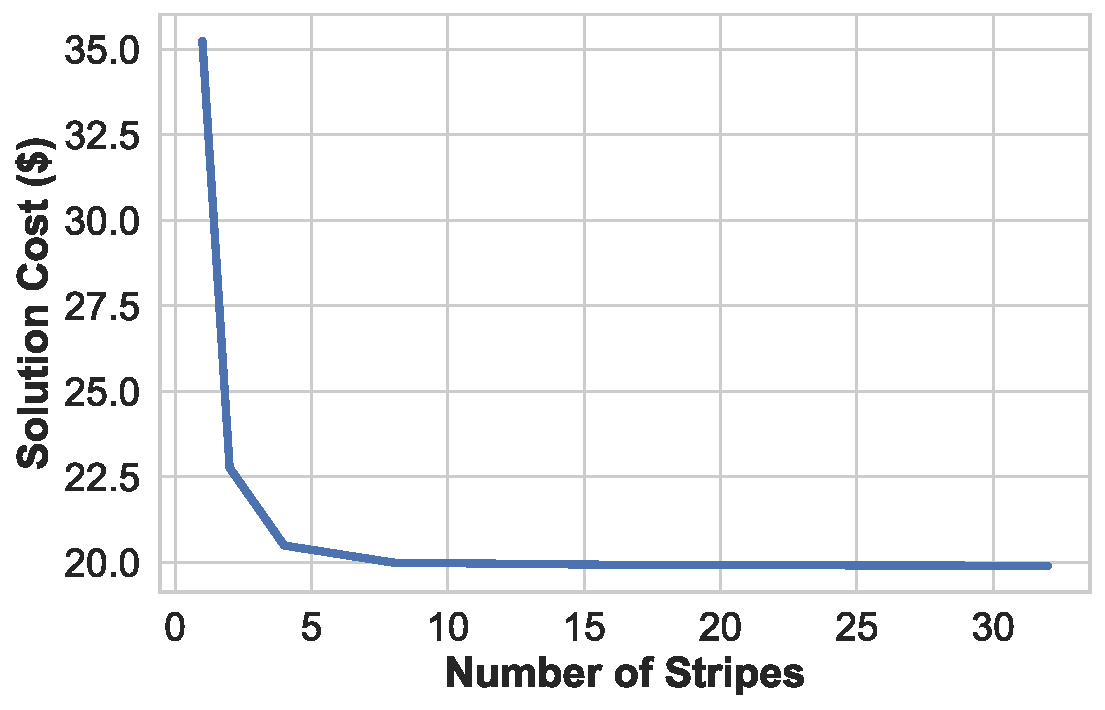
\includegraphics[width=.85\linewidth]{figures/num_stripes_quality.pdf}
    
    \caption{\textbf{Solution quality v.s the number of stripes.} Given a 6-destination intra-AWS transfer job and the same runtime SLO, our optimizer generates different solutions for different numbers of stripes. Small numbers of stripes can result in no feasible solution or solution with worse quality (i.e., higher cost). However, increasing the number of stripes to larger than 10 has diminishing returns.}  
    
    \label{fig:stripe-quality}
\end{figure} 

\subsection{Node Sub-Selection}
In Figure \ref{node-filtering}, we describe how we cluster nodes to select a subset of nodes for consideration by the optimizer. We motivate this by running an experiment to randomly select a subset of nodes in Figure \ref{fig:node_selection}. Generally, there are diminishing returns (beyond 20 nodes) to consider additional nodes. To avoid variability from randomness, we use the techniques described in  Figure \ref{fig:node_selection} to select a represented subset of nodes. 

\begin{figure}[ht]
     % \centering
     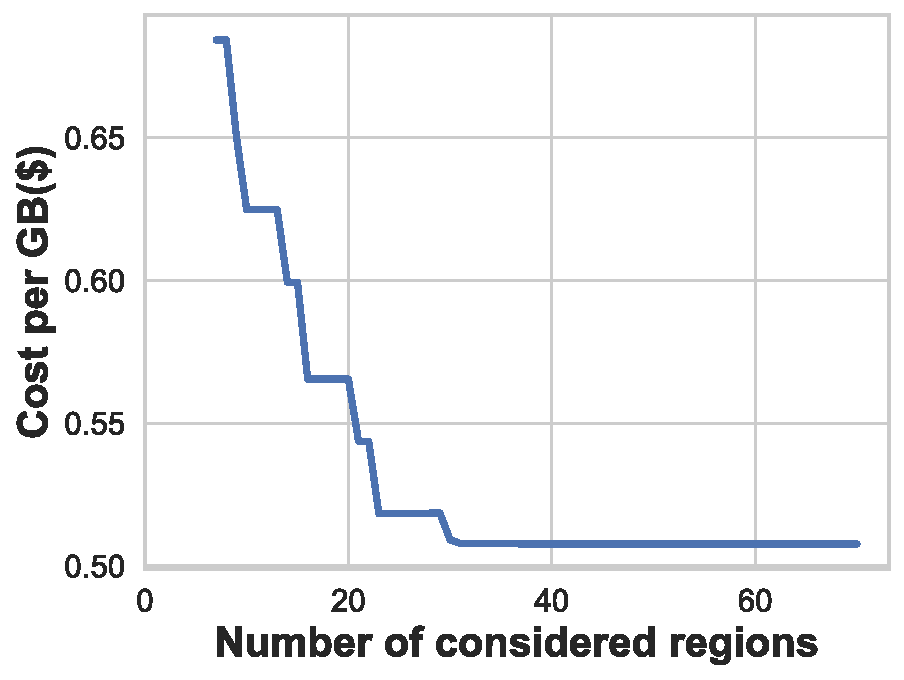
\includegraphics[width=.65\linewidth]{figures/node_sensitivity.pdf}
     \caption{Solution quality versus the number of considered nodes. Considering a larger set of regions has diminishing returns of solution quality but exponentially increases optimizer runtime. \shu{can move this graph to either the appendix, or replace it by \# of cluster ablations}}
     \label{fig:node_selection}
\end{figure}


\section{Formulation Details}
\label{s:formulation-details}

\subsection{Ensuring Valid Paths}
We cannot ensure connectivity of prevent cycles in paths defined by $\indicator$ without adding an exponential number of constraints. We define a special flow variable $\flow$ to add constraints that ensure that flow can be pushed along paths from $\indicator$ from the source to all destinations.\ion{I really think that for the entire subsection~\ref{sec-optimizer} we need to have a working example and refer to it throughout the section. Otherwise, it is hard to follow, like this para!}  The source node is denoted as the source region index in the transfer, the destination nodes are denoted as the destination region indices, and the sink node is denoted as a special node that is only connected to destination nodes. 
%
We constrain $\flow$ to have flow~\ion{What does it mean "$\flow$ to have flow"?} if and only if the corresponding stripe and edge for $\indicator$ is set to $1$. 
\begin{equation}
    \flow_{s, (u,v)}  \ge 1, \text{ if } \indicator_{s,(u,v)} = 1
\end{equation}
We ensure zero or negative flow 
\joey{I am confused, why would we have negative flow? What does that mean? Is the reverse of a flow negative?}
for $\indicator_{s,u,v} = 0$ via capacity constraints. We set special capacity constraints between destination nodes and the sink, to ensure that the sink can only receive sufficient flow if it receives flow from all destinations. 
\joey{I am having trouble getting an intuition for flow. Can you provide more high-level intuition?}\ion{Where is $\dest$ defined? I assume is the set of destinations. And, yes, the definition is confusing. Again, and running example in this section would help a lot.} 
\begin{equation}
    \flow_{s, (u, v)} \le 
\begin{cases}
    1,& \text{if } u\in \dest, v= \text{sink} \\
    0,& \text{if } \indicator_{s,(u,v)} = 0 \\
    |\dest|,              & \text{otherwise}  
\end{cases}
\end{equation}
We impose conservation of flow $\forall s$:\ion{Hard to reconcile above and below equations.}  
\begin{equation}
    \sum_{u\in V} \flow_{s, (u, v)} = 
\begin{cases}
    |\dest|,& \text{if $v$ is the source \shu{Why v?}} \\
    -|\dest|,              & \text{if $v$ is the sink}  \\
    0,              & \text{otherwise}
\end{cases}
\end{equation}
\joey{It occurs to me, is this graph directed?  Does $F_{s,u,v} = -F_{s,v,u}$?}
\joey{I really think this entire sub-section (5.2) should start with the idea that we will frame this problem as a MILP on a directed graph (or something).}
If the above constraints are met, this ensures that the stripe paths assigned by $\indicator$ are able to push flow from the source to all destinations. 

\subsubsection{Full Formulation}
We can write a full formulation of an integer linear program as the following: 
\begin{flalign}
& \argmin_{\indicator,\instances, \flow}  \runtime * \frob{\costi} \instances + \sum_s  \frob{\coste} \indicator \\
    & \instances \le \maxinstances \\
    & \stripesize * \sum_{s} \indicator_{s,(u, v)} \le \capacitye_{u, v} \\
    & \stripesize * \sum_{s}\sum_{u\in V} \indicator_{s, (v, u)} \le \capacityiegress \\
    & \stripesize * \sum_{s}\sum_{v\in V} \indicator_{s, (v, u)} \le \capacityiingress \\
    & \flow_{s, (u, v)}  \ge 1, \text{ if } \indicator_{s,(u,v)} = 1 \\
    & \sum_{u\in V} \flow_{s, (u, v)} = 
\begin{cases}
    |\dest|,& \text{if $v$ is the source} \\
    -|\dest|,              & \text{if $v$ is the sink}  \\
    0,              & \text{otherwise}
\end{cases} \\
    & \flow_{s, (u, v)} \le 
\begin{cases}
    1, &\text{if } u\in \dest, v= \text{sink} \\
    0, &\text{if } \indicator_{s,(u,v)} = 0 \\
    |\dest|,              & \text{otherwise}  
\end{cases}
\end{flalign}



%  \begin{figure}[t]
%      \centering
%      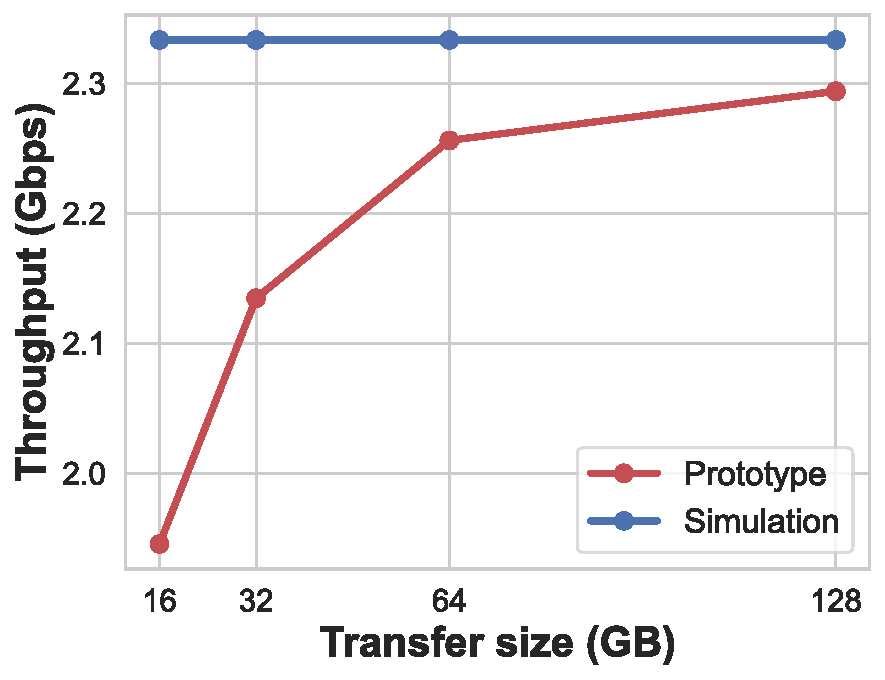
\includegraphics[width=.75\linewidth]{figures/new_simulator_accuracy.pdf}
%      \caption{Actual throughput v.s Predicted throughput: Throughput profiles can be used to accurately predict the throughput of data distribution trees. Here
% shows the result of the simulation and prototype through-
% put comparisons for 6-dest transfer \sarah{make this percentage} \sarah{DUPLICATE WITH TABLE}
%      }\label{fig:simulator_accuracy}
% \end{figure}

\section{How does Cheaper Egress Affect \sys's Optimizations?}
Some existing cloud providers (e.g., Cloudflare \cite{cloudflareegress}, Wasabi \cite{wasabi}, and Blackblaze \cite{blackblaze}) offer discounted or even free network egress.
Interestingly, incorporating free-egress clouds into \sys offers further opportunities to reduce costs.
Figure \ref{fig:cloudflare} illustrates this effect.
This highlights the importance of using a system like \sys, which can adapt replication plans in response to cheaper network offerings.

It is possible that major cloud providers will also adapt free-egress models or, in a less extreme case, make intra-cloud network fees more uniform as they build up additional capacity for inter-region networks with limited bandwidth. In this case, the techniques used by \sys{} (overlay networking, VM parallelism, and striping) would achieve only substantial throughput improvements but no cost improvement.

% \begin{figure}[t!]
%     \centering
%     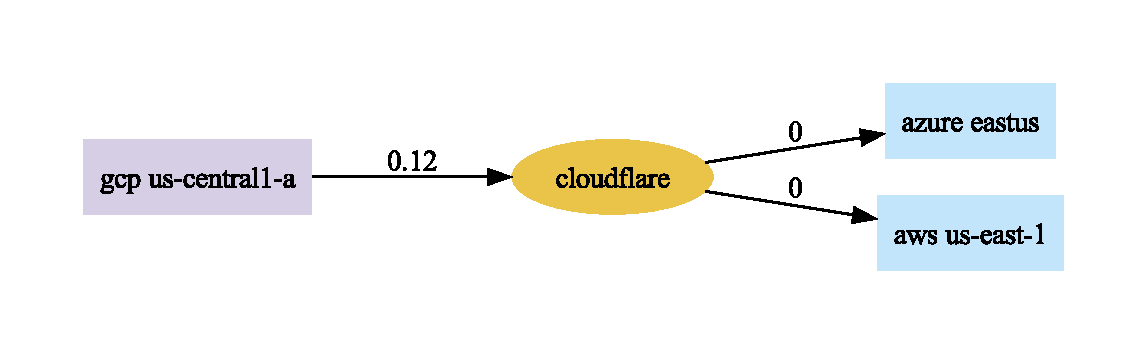
\includegraphics[trim=1cm 1.25cm 1cm 1.25cm, clip, width=\linewidth]{figures/cloudflare.pdf}
%     \caption{Routing data through free-egress clouds (e.g., Cloudflare): Inter-cloud egress only needs to be paid \textit{once} rather than a minimum of \textit{twice} to replicate data across three cloud providers (AWS, GCP, and Azure).}
%     \label{fig:cloudflare}
% \end{figure}

% \begin{table}[tbp]
% \caption{For the example in Figure~\ref{fig:cloudflare}, it is 2$\times$ cheaper to route via Cloudflare with Cloudcast.}
% \begin{tabular}{|l|l|l|l|}
% \hline
%  & \textbf{Direct} & \textbf{Cloudcast} & \textbf{\begin{tabular}[c]{@{}l@{}}Cloudcast \\ (with Cloudflare)\end{tabular}} \\ \hline
% \textbf{Cost (\$/GB)} & 0.24 & 0.2075 & 0.12 \\ \hline
% \end{tabular}
% \end{table}

\begin{figure}[ht!]
    \centering
    \begin{subfigure}[t]{0.5\textwidth}
        \centering
        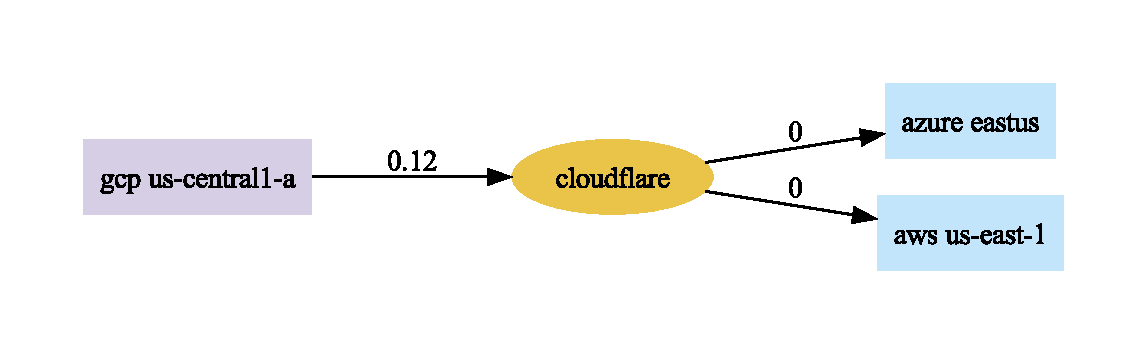
\includegraphics[trim=1cm 1.25cm 1cm 1.25cm, clip, width=\linewidth]{figures/cloudflare.pdf}
        \caption{Example of routing via no egress fee clouds.}
        \label{fig:cloudflare}
    \end{subfigure}

    \vspace{8pt}

    \begin{subfigure}[t]{\columnwidth}
        \centering
        \small
        %\resizebox{\textwidth}{!}
        \caption{Egress cost is 2$\times$ cheaper including Cloudflare in Cloudcast.}
        \label{tab:cloudcast}
    \end{subfigure}

    \vspace{8pt}
    
    \caption{Routing data through clouds with no egress fees (e.g., Cloudflare) can reduce inter-cloud replication costs as egress fees need to be paid only \textit{once} rather than a minimum of \textit{twice} to replicate data across AWS, GCP, and Azure.}
    \label{fig:table_figure}
\end{figure}